\newcommand{\st}{ \ | \ }

\section{Graph-Based Syntax Definition and Formalisms}
  \label{s:syntax definition}
  In this section we present our graph-based syntax, beginning with the necessary graph 
  theoretic fundamentals to construct the graphs discussed in Sec.~\ref{s:requirements}. 
  The notation used in this paper is adapted from Diestel \cite{Diestel2010}. 
  A \emph{graph} is a pair $G = (V,E)$ of sets such that $E \subseteq V \times V$, 
  which means that the elements of $E$ are 2-element subsets of $V$. The set $V$ 
  contains the \emph{vertices} or \emph{nodes} and the set $E$ contains the \emph{edges}.
  For a \emph{directed graph} (or \emph{digraph}) we construct $E$ as a set of ordered pairs instead 
  of a set of sets. Each ordered pair represents an edge starting at the node 
  indicated by the first entry and directed to the node indicated by the second 
  entry. An edge $e$ = $(x,y)$ may simply be referred to as $xy$. The edges 
  directed out from node $v$ are denoted by $E(v)$ and the edges directed into $v$ are denoted 
  by $E^{-1}(v)$. $E(v)$ may be the empty set, a single edge, or a set of edges, and likewise for $E^{-1}(v)$.
  \begin{figure}[htb!]
    \begin{center}
    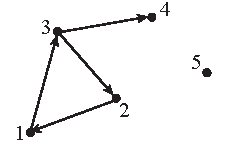
\includegraphics[width=1.5in]{images/example_directed_graph}
    \end{center}
    \vspace{-20pt}
  \caption{Example directed graph.}
  \label{f:example directed graph}
  \end{figure}
  As an example, for the directed graph shown in Fig.~\ref{f:example directed graph} we have
  \begin{IEEEeqnarray*}{rCl}
  V & = & \{1,2,3,4,5\}, \\
  E & = & \big\{(2,1),(3,2),(1,3),(3,4)\big\}.
  \end{IEEEeqnarray*}

  A \emph{path} $P=(V,E)$ from $x_0$ to $x_k$ in graph $G$ is a subgraph of $G$ 
  with $V = \{x_0,x_1,\ldots,x_k\}$ and $E = \{(x_0,x_1),(x_1,x_2),\ldots,(x_{k-1},x_k)\}$. 
  Path $P$ is a \emph{cycle} if $x_0 = x_k$.
  A \emph{reverse path} $P_R$ in graph $G$ is a path on $R$, where $R$ is the 
  reverse graph of $G$ obtained by switching the orientation of every edge.


  %does this belong in the analysis block section???? 
  Let $I$ be a nonempty set such that for each $i \in I$ there is a corresponding set $A_i$. 
  The set of sets $\mathcal A = \{A_i \st i \in I\}$ is called an indexed family of sets with index $i$ and 
  indexing set $I$ \cite{smith2006}. 
  The union over this family of sets can be described in a few different ways:
  \begin{equation}
  \bigcup_{i \in I} A_i = \bigcup_{A \in \mathcal A} A = \{x \st x \in A \txt{ for some } A \in \mathcal A\}.
  \end{equation}

  Lastly, the cardinality of a set $B$ is the number of elements in $B$ and is denoted as $|B|$.

\subsection{Node and Edge Types}
  \label{ss:types}
We categorize nodes and edges 
  into distinct types in order to provide an intuitive approach to MDAO problem formulation. 
  The three node types are
    \begin{description}
      \item[\bf{variable node:}] represents scalar or array data, inputs and outputs,
      \item[\bf{function node:}] represents the computation performed by analysis tools,
      \item[\bf{driver node:}] represents control logic capable of managing iterations 
      (present only in a PSG),
    \end{description}
  and the three edge types are

  \begin{description}
  \item[\bf{connection edge:}] represents exchange of information external to analysis tools,
  \item[\bf{function edge:}] represents exchange of information internal to analysis tools,
  \item[\bf{driven edge:}] represents passing of information from a driver node to a 
  variable node (present only in a PSG).
  \end{description}
  Figure \ref{f:sellar types} demonstrates the usage of these node and edge 
  types via the Sellar problem. 
In this figure, function nodes are indicated by squares, 
  variable nodes are indicated by circles, connection edges are indicated by 
  dotted lines, and function edges are indicated by solid lines.
  \begin{figure}[htb!]
    \begin{center}
      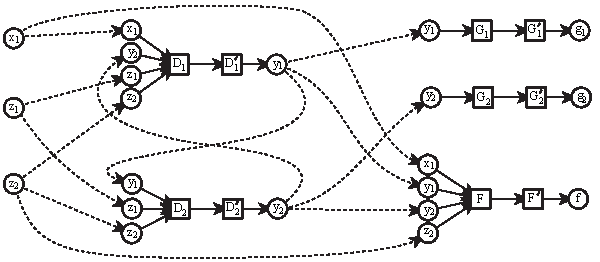
\includegraphics[width=3.25in]{images/sellar_types}
    \end{center}
    \caption{Sellar problem represented as a graph.}
  \label{f:sellar types}
  \end{figure} 

  A rule set is provided for the usage of these node and edge types to provide a structure 
  to the graph-based representation. The driver node and the driven edge are allowed only in 
  PSGs, whereas the other node and edge types can be present in any of the three graph types, 
  subject to the following restrictions: 
  \begin{enumerate}
  \item A function node may have only one edge directed to or from another function node.
  \item A function node may have only function edges directed in or out.
  \item A function node must have at least one edge directed in and at least one edge 
    directed out.
  \item If a variable node has an outgoing function edge, then it may not have other 
  outgoing edges.
  \item If a variable node has an incoming function edge, then it may not have any 
  additional incoming edges.
  \end{enumerate}

 Alexandrov and Lewis's REMS syntax includes only two node types (variable and function) 
  and one edge type   \cite{alexandrov2004}. The present work adds one additional 
  node type and two additional edge types to the syntax to allow descriptive
  graphs for all three phases of the design problem formulation process discussed 
  in Sec. \ref{s:requirements}.

\subsection{Analysis Blocks}
\label{ss:analysis blocks}
  Analysis tools take in a set of input variables and calculate 
  the values for their respective outputs. We represent this process
  by a digraph called an \emph{analysis block}; a notional analysis block is shown 
  in Fig.~\ref{f:analysis block}. 
  %Each analysis block is a directed graph denoted as $ A=(V_{A},E_{A})$
  As indicated in this figure, analysis blocks comprise three sets of nodes 
  representing the distinct local inputs, the analysis (computation), and the 
  distinct local outputs. The local input and local output nodes are variable 
  nodes, while the nodes representing the analysis are function nodes. All of 
  the edges within the analysis block are function edges, and are considered 
  fixed to the analysis block. This graph structure demonstrated by 
  Fig.~\ref{f:analysis block} satisfies the rules listed in Sec.~\ref{ss:types}. 
  Conversely, the rules ensure that analysis tools are represented via this analysis 
  block structure.

  \begin{figure}[htb]
      \begin{center}
      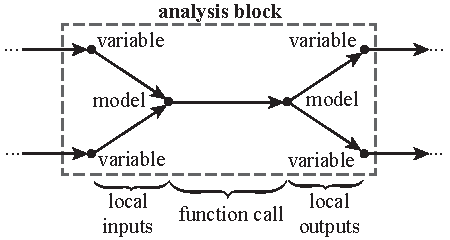
\includegraphics[width=3.0in]{images/analysis_block}
      \end{center}
      \vspace{-10pt}
  \caption{Example analysis block with node types labeled.}
  \label{f:analysis block}
  \end{figure}

  The function edge connecting the two function nodes represents the necessary 
  calculations to map the inputs to the outputs of the analysis. 
  This edge also provides the opportunity to encode computational cost or other 
  characteristics of the analysis code as a weight in a weighted graph formulation. 
  Because all the edges within analysis blocks are fixed, the blocks themselves are fixed 
  sub-graphs within the overall MDAO problem graph. 
  The connectivity of nodes and edges in an analysis block cannot be altered for the 
  purposes of MDAO problem formulation; 
  however, analysis block sub-graphs can be added or removed from the MDAO problem 
  graph as needed. Variable nodes in an analysis block can be distinguished as either an 
  input or an output by the manner in which they are connected. As shown in 
  Fig.~\ref{f:analysis block}, inputs are represented as variable nodes that have an 
  outgoing edge into a function node, and outputs are represented as variable nodes that 
  have an incoming edge from a function node. 

\subsection{Objectives, Constraints, and Inputs}
  \label{ss:objectives and constraints}
  Along with analysis tools, objectives, constraints, and inputs also need to be represented.
  In the case of objective functions, a single output value generated by an analysis 
  block could be selected, but commonly, multiple output values from different analysis 
  tools are aggregated together to form a composite objective function. 
  Generally, both objective and constraint functions accept a set of inputs and map them 
  to an output value of significance to the overall design problem. 

  The operations of implementing composite objective and constraint functions, 
  although typically simple, are effectively identical to the task performed by an analysis block. 
  A composite constraint or objective function can therefore be represented as an 
  analysis block within the graph with its own input and output variable nodes. 
  Although fundamentally no different than an analysis block, for clarity and 
  convenience, it is useful to distinguish between analysis blocks corresponding to 
  analysis codes and those that arise from the addition of objectives or constraints to the graph. 
  Therefore, we use an \emph{expression block} to represent an objective or constraint. 
  These expression block graphs follow the same structure as analysis blocks 
  presented in Sec.~\ref{ss:analysis blocks}.

  Finally, inputs to the problem formulation are represented in the graph by individual 
  variable nodes with connection edges directed out to corresponding local inputs of 
  analysis blocks, and they are referred to simply as \emph{inputs}. 
  These nodes serve to indicate that the variable nodes within analysis or 
  expression blocks to which they are connected represent the same variable in the 
  problem formulation.

  Figure \ref{f:obj-cons} demonstrates the use of inputs (black circles), analysis 
  blocks (dotted boxes), and expression blocks (dashed boxes), for the Sellar problem 
  graph.
  \begin{figure}[htb!]
    \begin{center}
      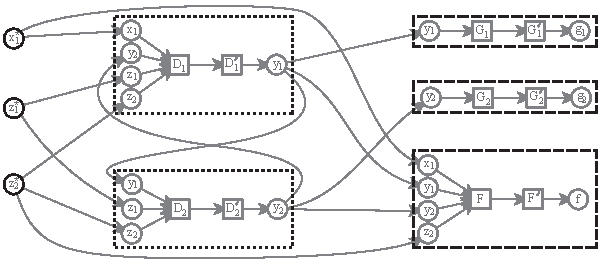
\includegraphics[width=3.25in]{images/sellar_obj_and_cons}
    \end{center}
    \caption{Sellar problem graph indicating inputs (black circles), analysis blocks 
    (dotted boxes), and expression blocks (dashed boxes).}
  \label{f:obj-cons}
  \end{figure} 

\subsection{Indegree and Outdegree Limits}
  \label{s:indegree-outdegree}
	To address the MDAO notion of design variables, we first introduce the concept of the 
  degree of a node. In a digraph, \emph{indegree} of a node is the number of edges 
  directed in and is denoted as $\txt{deg}^-(v)$, and the \emph{outdegree} 
  is the number of edges directed out and it is denoted as $\txt{deg}^+(v)$ \cite{Diestel2010}.

  We may now define the \emph{upper indegree limit} 
  \begin{equation}
  \txt{deg}_u^-(v):V \to \mathbb{N}
  \end{equation} 
  and the \emph{lower indegree limit} as
  \begin{equation}
  \txt{deg}_l^-(v):V \to \mathbb{N}.
  \end{equation}
  These user-specified limits govern the number of connection edges that may 
  be directed into a node for a valid graph; of course, the specification must 
  satisfy $\txt{deg}_l^-(v) \leq \txt{deg}_u^-(v)$.
  For example, consider a variable node $v$ with $\txt{deg}_u^-(v) = \txt{deg}_l^-(v) = 1$. 
  In this case, $v$ must have exactly one incoming connection edge or the graph is 
  deemed an invalid problem formulation. 


  \subsection{Driver Nodes and Driven Edges}
  Within this syntax, all iterative processes are represented with Driver nodes. 
  The driver node shares some basic qualities with the model node. It can have incoming 
  and outgoing function edges to and from variable nodes. For example, many optimizers take 
  convergence tolerance as input and output iteration counts and final objective value. 
  With respect to variable nodes and function edges, drivers behave exactly the same as
  model nodes and are subject to the same rules governing their use in the graph. In this
  context, driver nodes can be part of driver blocks which behave just like analysis 
  blocks. 

  Driven edges are the distinguishing characteristic associated with driver nodes and
  driver blocks. Driven edges don't follow the same rules as other edges. Driven edges  
  will always connect a driver node to a variable node (in either direction), but they 
  are not considered when counting the indegree or outdegree of the variable node.
  Hence a single variable node could have multiple incoming driven edges from different 
  driver blocks. Figure \ref{f:driver block} shows a notional example where a driver block 
  represents and optimizer solving an unconstrained minimization problem. 

  \begin{figure}[htb]
    \begin{center}
    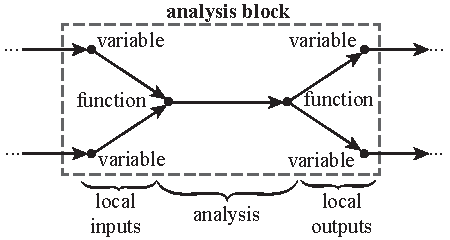
\includegraphics[width=3.0in]{images/driver_block}
    \end{center}
    \vspace{-10pt}
  \caption{Example driver block with node types labeled.}
  \label{f:driver block}
  \end{figure}


\section{MDAO Constructs Derived from the Graph-Based Syntax}
  \label{s:graph representation}
  In Sec.~\ref{s:syntax definition}, we presented the structure of the graph-based 
  representation. We now discuss how these formalisms provide the remaining MDAO problem 
  constructs identified in Sec.~\ref{s:requirements}.

\subsection{Design Variables, Holes, and Collisions}
  Design variables are input variables whose values are free to be 
  changed by the designer or by an optimizer in an MDAO study. In the graph-based 
  syntax, a node corresponds to a design variable if the indegree limits of the node are 
  prescribed as zero.

  If the indegree limits are violated by the number of incoming connection edges 
  (the indegree of the node), then the graph is regarded as an invalid problem formulation. 
  There are two classifications for these violations:
    \begin{description}
      \item[\bf{hole:}] The number of incoming edges is less than the lower indegree limit:
        \begin{equation} 
          \txt{deg}^-(v) < \txt{deg}_l^-(v). 
          \label{e:hole} 
        \end{equation}
        A hole represents a lack of information being supplied to the variable node. 
        This implies that the analysis tool being represented by the analysis block 
        would not be capable of producing outputs.
      \item[\bf{collision:}] The number of incoming edges is greater than the upper 
      indegree limit:
        \begin{equation} 
        \txt{deg}^-(v) > \txt{deg}_u^-(v). 
        \label{e:collision}
        \end{equation}A collision represents redundant information being supplied to 
        the variable node from two or more sources. This conflict implies an 
        ambiguity as to which information is to be used as an input for the analysis tool.
	In multifidelity problems (discussed subsequently), the upper indegree limit could be 
  specified as $deg_u^- > 2$, which implies that a collision is not noted in the case of 
  multiple inputs.
  \end{description} 

  The presence of holes and collisions in a graph represent conflicts that will give
  rise to an invalid problem formulation. The process of obtaining an FPG from an 
  MCG will reveal these conflicts.

\subsection{Coupling Between Analyses}
  In MDAO, coupling is the mutual dependence between two or more analysis 
  tools and their respective outputs. In this graph-based syntax, coupling is 
  described by the presence of a cycle between two or more analysis blocks. In the Sellar 
  problem from Eq.~\ref{eqn:simple_fpf} 
  a mutual dependence between $D_1$ and $D_2$ exists through the variables $y_1$ and $y_2$. 
  The edges belonging to a cycle in the Sellar problem are highlighted in 
  Fig. \ref{f:sellar cycles}.  These edges collectively form a closed path between 
  analysis blocks $D_1$ and $D_2$.

  \begin{figure}[htb!]
    \begin{center}
      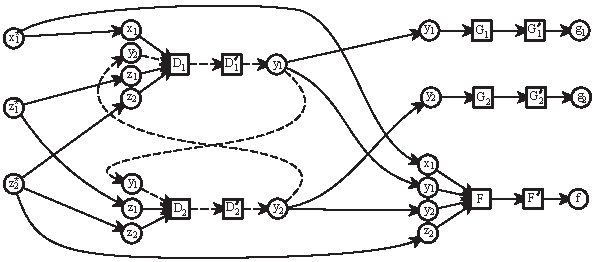
\includegraphics[width=3.25in]{images/sellar_cycles}
    \end{center}
    \caption{Sellar problem graph with dashed edges indicating %
    participation in a cycle.\label{f:sellar cycles}}
  \end{figure} 

  Coupling cycles do not contain driver nodes in the MCG or FPG representation. 
  Solvers, optimizers, and other iterative processes are not invovled in the coupling 
  definition; however, one or more solvers will be required to build a valid PSG from a 
  given FPG  that includes cycles. Additionally, a coupling cycle has no inherent 
  start or end point. It would be acceptable to select a
  node in the cycle as a starting point and proceed around the
  loop until the starting point is reached again. For the Sellar Problem, selecting 
  $D_1$ as the starting point would yield a problem as given in 
  Eq.~\ref{eqn:simple}.
  Larger problems can involve more complex cycles in their FPG, indicating more 
  complex coupling between analyses. For example, a cycle can involve more than 
   two analysis blocks. Multiple independent cycles could also exist, indicating 
  independent coupling relationships. Cycles can also overlap, meaning that the same analysis 
  blocks are involved in multiple different coupling cycles. All of these situations
  arise naturally as the size of problems grows, and managing this coupling may
  become difficult. In the present work, Sec.~\ref{s:example problem}
  demonstrates how building an FPG from an MCG provides an opportunity to 
  identify and potentially reduce the number of cycles in a graph. 

  If many couplings are present, convergence rates can be improved by 
  searching for an effective ordering for the execution of analyses.
  Rogers' DeMAID tool uses a genetic algorithm to find an ordering that minimizes 
  the overall coupling of the system by separating independent cycles in the 
  graph \cite{rogers1996,rogers1996demaid}. Rogers work focused on the matrix 
  form of the DSM for ordering optimization. Lu and Martins more recently leveraged 
  a weighted form of the DSM and used an iterative clustering approach to perform a 
  similar task to DeMAID \cite{Lu2012}.

\subsection{Multi-fidelity Problems}
  \label{ss:multi-fideliy problems}
  A multi-fidelity MDAO problem can be characterized by a formulation in which 
  two or more different analyses each calculate the same data. Multi-fidelity 
  is represented in a graph by a variable node having an indegree greater than 
  one, which means that multiple connection edges are directed into it. When the 
  upper indegree limit of a variable node is set above one, then the node is 
  implied to allow multiple fidelity instances of the variable. When the lower 
  indegree limit of a variable node is set above one, then multiple fidelity instances are required.

  In a multi-fidelity problem, a given variable node may have multiple incoming 
  edges without implying a collision as defined by Eq.~\ref{e:collision}. 
  Figure \ref{f:collision_example} shows a modified version of the Sellar problem 
  with a new analysis, $D_0$, representing a low fidelity version of $D_1$. 
  In this modified version, the variable nodes with an upper indegree limit of two 
  are highlighted in gray, and changing the upper indegree limits for the variable nodes 
  representing $y_1$ in $D_2$, $F$, and $G_1$ avoids a collision. In Sec.~\ref{ss:obtaining FPG} 
  we present an algorithm for locating conflicts within a given MCG such that a designer 
  can make the necessary decisions about each one in turn. 
  \begin{figure}
    \begin{center}
      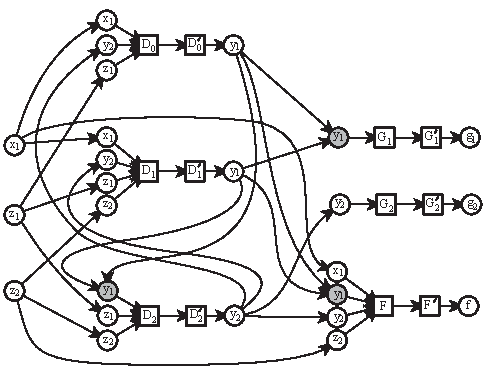
\includegraphics[width=3.25in]{images/sellar_mulfi}
    \caption{Graph of the modified Sellar problem with multi-fidelity nodes highlighted in gray.\label{f:collision_example}}
  \end{center}
  \end{figure}

  Multi-fidelity problems are always characterized by graphs in which at least some of the variable 
  nodes that have an $\txt{deg}^-_u(v) > 1$. These problems require 
  special techniques for resolving the conflicting edges by introducing some mechanism
  to manage when each of the different fidelity analyses are 
  run \cite{march2012provably,alexandrov2001approximation,Huang_Allen_Notz_Miller_2006}.
  The specifics of this mechanism are not represented within an MCG or 
  FPG. Instead, the multi-fidelity mechanism specifics would be represented as a 
  driver in a PSG derived from a multi-fidelity FPG. 

Table \ref{t:variable node classification} summarizes the classification of a variable 
node as a hole, design variable, single valid input (nominal), collision, or 
multi-fidelity node.

\begin{table}[htbp]
  \centering
  \caption{Variable Node Classification}
    \begin{tabular}{ccccc}
    \toprule
    $\txt{deg}^-_l(v)$ & $\txt{deg}^-_u(v)$ & $\txt{deg}^-(v)$ & valid & classification \\
    \midrule
    0     & 0     & 0     & yes   & design variable \\
    0     & 0     & 1     & yes   & collision \\
    0     & 1     & 0     & yes   & design variable \\
    0     & 1     & 1     & yes   & single input \\
    1     & 1     & 0     & no    & hole \\
    1     & 1     & 1     & yes   & single input \\
    1     & 1     & $>1$ & no    & collision \\
    1     & 2     & 1     & yes   & supplied input \\
    1     & 2     & 2     & yes   & multi-fidelity \\
    2     & 2     & $<2$ & no    & hole \\
    2     & 2     & 2     & yes   & multi-fidelity \\
    2     & 2     & $>2$     & no   & collision \\
    \bottomrule
    \end{tabular}%
  \label{t:variable node classification}%
\end{table}%


\subsection{Iterative Control: Drivers}
  There are many iterative processes that are used to help solve MDAO problems such as 
  solvers, optimizers, and Design of Experiment (DOE). Abstractly, even a human picking 
  values guided by experience and trend could be viewed as an iterative process. 
  These processes represent the control structures that govern how a design problem 
  marches toward a solution but they do not fundamentally impact the definition of the 
  problem to be solved. e.g. which optimizer you choose does not change the problem you 
  are solving but will change the path you follow to solve it. Hence, as a rule, driver 
  nodes and driven edges are excluded from both the MCG and FPG which deal exclusively 
  with problem formulation. They only come into play with in the PSG where the issue of 
  how to solve a specific problem is addressed. In fact, at least one driver block is 
  required to be present in any PSG in order to select values for the design variables. 





